\documentclass[../../main.tex]{subfiles}

\graphicspath{{\subfix{../../immagini/}}}

\begin{document}
    Per il percettrone multistrato la struttura scelta è quanto più semplice possibile, pur cercando di mantenere delle buone prestazioni. Questa scelta deriva dall'utilizzo che poi avrà questo classificatore: se questo infatti verrà inserito all'interno di un filtro appreso, l'obiettivo è avere un modello il più piccolo possibile in termini di spazio e comunque con delle prestazioni accettabili.

    La figura \ref{fig:strutturaPercettrone} riassume la struttura del percettrone: la rete è formata da 3 strati, dove il numero di neuroni del livello di input dipende dalla codifica utilizzata per gli elementi del dataset (quelle utilizzate negli esperimenti verranno introdotte nel prossimo paragrafo), mentre il numero di neuroni dello strato nascosto è arbitrario; infine, lo strato d'uscita contiene un solo neurone con una funzione d'attivazione sigmoidea, e di fatto fornisce la probabilità che l'elemento in ingresso abbia come etichetta 1.

    La funzione di perdita da minimizzare, trovandoci in un problema di classificazione binaria, è la cross entropy loss, già definita nell'equazione \ref{eqn:logloss}.

    \begin{figure}[H]
        \centering
        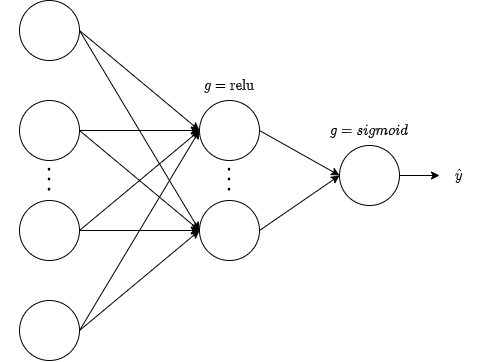
\includegraphics[width=\textwidth]{immagini/6_4/percettroneStruttura.drawio.png}
        \caption{}
        \label{fig:strutturaPercettrone}
    \end{figure}
\end{document}